\section{Local collision geometry}\label{sec:double}

\subsection{Event assumptions and a finite heat expansion}
Fix an interior point \((\tau_*,x_*)\) such that
\begin{equation}\label{eq:double}
 h=h_x=0,\qquad a=h_{xx}\ne0,
 \qquad b=h_{xxx},\quad c=h_{xxxx},
\end{equation}
with derivatives evaluated at that point unless stated otherwise.
This is a hypothetical event of the canonical family; its existence is
not assumed elsewhere. Since \(h(\tau,0)>0\), its position is nonzero.
Evenness gives a reflected event at \(-x_*\); the analysis is local
near either one.

Set \(s=\tau-\tau_*\), \(y=x-x_*\).
The heat equation replaces each time derivative by two spatial
derivatives. Taylor expansion therefore gives
\begin{equation}\label{eq:heat-four-jet}
 h(\tau_*+s,x_*+y)
 =\frac a2(y^2+2s)+\frac b6(y^3+6sy)
  +\frac c{24}(y^4+12sy^2+12s^2)+\mathcal R(s,y).
\end{equation}
For fixed compact sets in \((S,Y)\),
\(\mathcal R(\epsilon^2S,\epsilon Y)=O(\epsilon^5)\).
This notation assigns weight two to \(s\) and weight one to \(y\).
To justify it, take a sufficiently high finite Taylor expansion in
\((s,y)\). Terms of weight below two vanish by \eqref{eq:double};
the terms of weights two, three and four are exactly those displayed.
Every omitted monomial has weight at least five, and the ordinary
Taylor remainder has the same bound after rescaling. The source bounds
justify the needed finite derivatives. The constants depend on the event
and the chosen compact set.

\subsection{The regular critical curve}
\begin{proposition}[Critical-value crossing]\label{prop:critical}
There is a unique analytic local curve \(x_c(\tau)\) with
\(x_c(\tau_*)=x_*\) and \(h_x(\tau,x_c(\tau))=0\).
For \(v(\tau)=h(\tau,x_c(\tau))\),
\begin{equation}\label{eq:critical-exact}
 x_c'=-\frac{h_{xxx}}{h_{xx}},\qquad v'=h_{xx}
 \quad\hbox{along the curve}.
\end{equation}
Its expansions are
\begin{align}
 x_c(\tau_*+s)&=x_*-\frac ba s+O(s^2),\label{eq:critical-place}\\
 v(\tau_*+s)&=as+\frac12\left(c-\frac{b^2}{a}\right)s^2+O(s^3).
 \label{eq:critical-value}
\end{align}
\end{proposition}
\begin{proof}
Apply the analytic implicit-function theorem to \(h_x\), whose spatial
derivative at the event is \(a\ne0\). Differentiating \(h_x=0\) along
the curve gives \(h_{xxx}+h_{xx}x_c'=0\). Differentiating \(v\) gives
\(v'=h_\tau+h_xx_c'=h_{xx}\). A second differentiation at the event
yields \(v''=h_{xxxx}+h_{xxx}x_c'=c-b^2/a\), proving the expansions.
\end{proof}

Thus the extremum value crosses zero transversely, with finite velocity
\(a\). If \(a>0\), it is a local minimum which rises through zero; if
\(a<0\), it is a local maximum which falls through zero. This description
remains regular at the event.

\subsection{The two-root cluster}
\begin{theorem}[Square-root splitting and drift]\label{thm:splitting}
In a sufficiently small fixed complex disk about \(x_*\), the field
has exactly two zeros counted with multiplicity for all sufficiently
small real \(|s|\). They satisfy
\begin{equation}\label{eq:roots}
 z_\pm(\tau_*+s)=x_*-\frac{2b}{3a}s+
 \begin{cases}
  \displaystyle\pm\sqrt{-2s}+O(|s|^{3/2}),&s<0,\\[2pt]
  \displaystyle\pm\ii\sqrt{2s}+O(s^{3/2}),&s>0.
 \end{cases}
\end{equation}
They are real and simple for \(s<0\), and a nonreal conjugate pair for
\(s>0\). Their midpoint is analytic in \(s\).
\end{theorem}
\begin{proof}
At \(s=0\) the zero has exact order two. Choose a disk containing no
other zero and having a nonzero boundary. Uniform analytic convergence
on that boundary preserves the zero count for small complex \(s\).
Put \(s=-t^2/2\), \(y=tY\). The quotient
\[
 t^{-2}h(\tau_*-t^2/2,x_*+tY)
\]
extends holomorphically to \(t=0\), with value
\(a(Y^2-1)/2\). The analytic implicit-function theorem at its simple
roots \(Y=\pm1\) supplies two analytic branches. Substitution in
\eqref{eq:heat-four-jet} gives
\begin{equation}\label{eq:t-roots}
 y_\pm(t)=\pm t+\frac{b}{3a}t^2+O(t^3).
\end{equation}
For real \(t\), the branches are real by conjugation and uniqueness.
For \(s>0\), take \(t=\ii\sqrt{2s}\); the leading imaginary parts are
nonzero and the roots are conjugate. Replacing \(t\) by \(-t\)
interchanges the two roots, so their sum and product are even analytic
functions of \(t\), hence analytic in \(s\). This also proves the
midpoint assertion and \eqref{eq:roots}.
\end{proof}

In increasing imaginary time, the real roots approach, meet and leave
the real axis. The direction is reversed in Newman \(\lambda\).
The total local complex multiplicity stays two. This is the standard
local forward-parabolic pattern \cite{Angenent1991}; a global zero count
on the whole line is not inferred from the local statement.

\begin{figure}[ht]
\centering
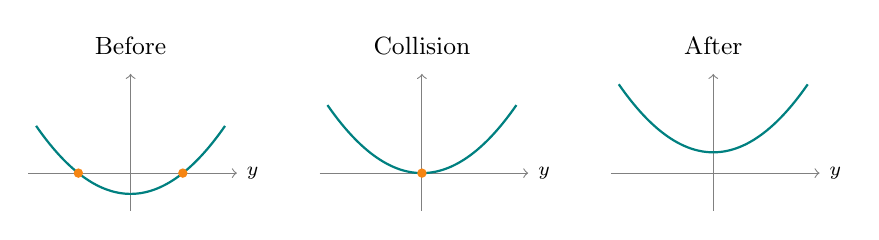
\begin{tikzpicture}[x=1cm,y=1.2cm]
 \foreach \shift/\ss/\title in {0/-0.22/Before,3.7/0/Collision,7.4/0.22/After}{
  \begin{scope}[xshift=\shift cm]
   \draw[->,gray] (-1.3,0)--(1.35,0) node[right,black] {\(\scriptstyle y\)};
   \draw[->,gray] (0,-0.4)--(0,1.05);
   \draw[thick,teal,domain=-1.2:1.2,samples=70]
    plot (\x,{0.5*\x*\x+\ss});
   \node at (0,1.35) {\small\title};
  \end{scope}
 }
 \fill[BurntOrange] (-0.6633,0) circle (1.7pt);
 \fill[BurntOrange] (0.6633,0) circle (1.7pt);
 \fill[BurntOrange] (3.7,0) circle (1.7pt);
\end{tikzpicture}
\caption{The universal quadratic model \(h/a=y^2/2+s\), with increasing
imaginary time from left to right. It illustrates the local analytic
law and is not a plot of theta data.}
\label{fig:fold}
\end{figure}

\subsection{A regular squared gap and the surrounding factor}
The symmetric functions constructed above define a monic quadratic
factor. Local analytic factorization gives
\begin{equation}\label{eq:local-factor}
 h(\tau,x)=(x-z_-(\tau))(x-z_+(\tau))U(\tau,x),
\end{equation}
where \(U\) is analytic and nonzero near the event. One may obtain the
quadratic's coefficients from the contour integrals of
\(x^k h_x/h\) around the fixed disk, which are analytic in \(\tau\);
division removes precisely the two enclosed roots. The quotient is a
holomorphic unit, including at \(s=0\). This is the same local
factorization used in the earlier heat-multiplicity analysis
\cite{HeatMultiplicity}. No product over all zeros is required.

For \(s<0\), write \(r_\pm=z_\pm\), \(\delta=r_+-r_->0\), and
\(q=\delta^2\). Let \(g=U_x/U\).

\begin{proposition}[Pair motion and squared gap]\label{prop:gap}
On the real-pair side,
\begin{align}
 r_\pm'&=-\frac{2}{r_\pm-r_\mp}-2g(\tau,r_\pm),\label{eq:pair-motion}\\
 \delta'&=-\frac4\delta-2\bigl(g(\tau,r_+)-g(\tau,r_-)\bigr),\label{eq:delta}\\
 q'&=-8-4q\int_0^1g_x(\tau,r_-+t\delta)\dd t.\label{eq:q-exact}
\end{align}
The squared gap extends analytically through the event and
\begin{equation}\label{eq:q-expansion}
 q(\tau_*+s)=-8s+16B_*s^2+O(s^3),\qquad
 B_*=\frac{c}{6a}-\frac{b^2}{9a^2}.
\end{equation}
The midpoint has velocity \(-2b/(3a)\) at the event.
\end{proposition}
\begin{proof}
At a simple zero \(r\), implicit differentiation gives
\(r'=-h_{xx}/h_x\). Differentiating \eqref{eq:local-factor} twice
at \(r_\pm\) yields
\[
 \frac{h_{xx}}{h_x}(\tau,r_\pm)
 =\frac{2}{r_\pm-r_\mp}+2g(\tau,r_\pm).
\]
Subtracting proves \eqref{eq:delta}; multiplying by \(2\delta\) and
using the fundamental theorem of calculus gives \eqref{eq:q-exact}.
Analyticity of the symmetric functions makes \(q\) analytic.
At \(s=0\),
\[
 U(\tau_*,x_*+y)=\frac a2+\frac b6y+\frac c{24}y^2+O(y^3),
\]
so \(g_*=b/(3a)\) and \(g_{x,*}=B_*\).
The integral in \eqref{eq:q-exact} tends to \(B_*\); its symmetric
expansion is \(B_*+O(s)\), since the midpoint is \(O(s)\) from \(x_*\)
and \(\delta^2=O(s)\). Thus \(q'(0)=-8\) and \(q''(0)=32B_*\),
proving \eqref{eq:q-expansion}. Adding the two root equations cancels
their singular terms and gives the midpoint velocity \(-2g_*\).
\end{proof}

The critical point and root midpoint generally have different velocities:
\(-b/a\) and \(-2b/(3a)\). Individual zero velocities diverge as
\(|s|^{-1/2}\), whereas both collective coordinates remain regular.
The term \(-8\) in \eqref{eq:q-exact} is the universal terminal closing
rate of a separated collision. The regular factor affects drift
and subsequent terms; this is not a uniform estimate on its size.

Rodgers and Tao's zero dynamics and gap law have the corresponding
decomposition with the opposite Newman-time sign
\cite[Section~4, Theorem~4.16 and Lemma~4.18(i)]{RodgersTao2020}.
Their printed theorem uses principal-value sums on the paper's
contradiction interval \(\Lambda<t\leq0\). We do not extend that theorem
to a different interval or to arbitrary nonreal zero configurations.
The local derivation above requires only the analytic factor \(U\).


\subsection{Amplitude, drift and relative curvature}
The coefficients in \eqref{eq:critical-place}--\eqref{eq:critical-value}
separate naturally into the amplitude \(a\) and two quantities unchanged
by a nonzero constant rescaling of the field:
\begin{equation}\label{eq:beta-gamma}
 \beta=\frac ba,\qquad \gamma=\frac ca-\frac{b^2}{a^2}.
\end{equation}
At the event, \(x_c'=-\beta\), \(v'=a\), and \(v''=a\gamma\).
At the reflected event, \(a,\gamma\) are unchanged and \(\beta\)
changes sign. The critical curve is the curve of stationary points
\(h_x=0\), not a curve of zeros of \(h\).

\begin{proposition}[Curvature transport and an event coordinate]
\label{prop:curvature-transport}
Along a regular critical curve, set
\(A(\tau)=h_{xx}(\tau,x_c(\tau))\ne0\) and \(r_c=-v/A\).
Then
\begin{align}
 A'&=h_{xxxx}-\frac{h_{xxx}^2}{h_{xx}},\qquad
 \frac{d}{d\tau}\log|A|
 =\frac{h_{xxxx}}{h_{xx}}-\frac{h_{xxx}^2}{h_{xx}^2},
 \label{eq:A-transport}\\
 r_c'&=-1-r_c\frac{A'}{A}.\label{eq:rc-transport}
\end{align}
In particular \(r_c(\tau_*+s)=-s+\tfrac12\gamma s^2+O(s^3)\)
and \(r_c\sim q/8\sim\tau_*-\tau\) on the real-pair side.
\end{proposition}
\begin{proof}
Differentiate \(A\) along the curve and use
\(x_c'=-h_{xxx}/h_{xx}\) and \(h_\tau=h_{xx}\).
The quotient rule and \(v'=A\) give \eqref{eq:rc-transport}.
Finally \(v=as+a\gamma s^2/2+O(s^3)\) and
\(A=a+a\gamma s+O(s^2)\), proving the expansion and, with
\eqref{eq:q-expansion}, the comparison.
\end{proof}

Thus \(\gamma\) is the relative rate of change of the extremum's
curvature. The regular event coordinates describe the same crossing;
they do not impose independent restrictions on it.

At the collision slice use the local factor \(U\) in
\eqref{eq:local-factor}, and write
\begin{equation}\label{eq:ell-kappa}
 \ell=\frac{U_x}{U}(\tau_*,x_*),\qquad
 \kappa=\partial_x\!\left(\frac{U_x}{U}\right)(\tau_*,x_*).
\end{equation}
The derivatives of \(h=(x-x_*)^2U\) give
\(U_*=a/2\), \(U_{x,*}=b/6\), \(U_{xx,*}=c/12\). Therefore
\begin{equation}\label{eq:coefficient-dictionary}
 \boxed{\ \beta=3\ell,\qquad c/a=6(\kappa+\ell^2),\qquad
 \gamma=6\kappa-3\ell^2,\qquad B_*=\kappa.\ }
\end{equation}
The same exterior curvature controls the second-order gap correction
and, together with the drift, the second-order critical value.

\subsection{A conditional real-zero benchmark}
\begin{proposition}[Exterior inverse-square curvature]
\label{prop:LP-coefficients}
Suppose additionally that the collision slice belongs to the real
Laguerre--P\'olya class. If its product has Gaussian factor
\(\ee^{-\alpha z^2}\), \(\alpha\ge0\), and \(\{\rho_j\}\)
are its remaining zeros, with multiplicities, after the two at \(x_*\)
are removed, then
\begin{equation}\label{eq:LP-kappa}
 \kappa=-2\alpha-\sum_j\frac{1}{(x_*-\rho_j)^2}.
\end{equation}
For an even slice with \(x_*\ne0\),
\begin{equation}\label{eq:LP-gamma}
 \kappa\le-\frac{1}{2x_*^2},\qquad
 \gamma\le-\frac{3}{x_*^2}-\frac{\beta^2}{3}<0.
\end{equation}
\end{proposition}
\begin{proof}
The defining canonical product is
\(Cz^m\ee^{-\alpha z^2+d z}
\prod_j(1-z/\rho_j)\ee^{z/\rho_j}\), with real parameters and zeros,
and \(\sum_{\rho_j\ne0}|\rho_j|^{-2}<\infty\)
\cite[Definition~1.1]{Csordas2014PositiveKernels}.
After removing the pair at \(x_*\), take the second logarithmic
derivative. The linear exponential and regularizing linear terms
disappear, giving \eqref{eq:LP-kappa}. The sum converges absolutely
locally off the remaining zeros; only finitely many are nearby and
the distant terms are bounded by a constant times \(|\rho_j|^{-2}\).
Evenness supplies a double zero at \(-x_*\), whose contribution is
\(-2/(2x_*)^2\). All other terms are nonpositive. Equation
\eqref{eq:coefficient-dictionary} proves \eqref{eq:LP-gamma}.
\end{proof}

This is a conditional benchmark for an all-real slice, not an
unconditional theta estimate. The weaker assertion \(\gamma\le0\)
also follows from the derivative Laguerre inequality \(b^2-ac\ge0\).
For \(a>0\), \eqref{eq:LP-gamma} says that a rising minimum
decelerates; its transverse crossing remains possible. The polynomial
\((x^2-r^2)^2\) has \(\beta=3/r\), \(\gamma=-6/r^2\) at \(r\)
and attains the displayed reflected-pair bound. This is a check of
the sharp constant, not a canonical-source example.

The sign changes when exterior zeros need not be real. An exterior
conjugate pair \(d\pm\ii\eta\) contributes
\begin{equation}\label{eq:complex-exterior-curvature}
 -\frac{2((x_*-d)^2-\eta^2)}{((x_*-d)^2+\eta^2)^2}
\end{equation}
to the logarithmic curvature, which may have either sign. A collision
at an all-real boundary and a later collision among a nonreal
background therefore require different estimates. The local theory
neither assumes nor proves that the global Newman threshold is
attained at one finite collision.

Finally, a bounded exterior correction by itself cannot oppose the
terminal closing rate. If the integral in \eqref{eq:q-exact} has
absolute value at most \(C>0\), then
\(q'\le-8+4Cq\le-4\) whenever \(0<q\le1/C\).
If this bound and cluster isolation persist, the pair closes in
at most \(q(\tau_0)/4\) further imaginary time. Preventing entry
into that regime requires information in addition to boundedness
of the regular factor.
